\subsection{Results and discussion}\label{sec:m1:results}

\subsubsection{Tests}\label{sec:m1:results:tests}
    ~\cref{fig:m1:omega_tests} show the evolution of the density fractions with time. They sum to one across all times which was required. At early times the radiation density dominates (orange line). The intersection between the orange and green lines mark the radiation-matter equality, after which matter is the dominating density. Likewise, the intersection between the green and purple lines mark the matter-dark energy equality, where dark energy (manifested in the cosmological constant) become the dominating density. Time can thus be divided into three regimes; radiation dominated, matter dominated, and dark energy dominated eras, separated by black dotted lines in the plot. 
    \begin{figure}
        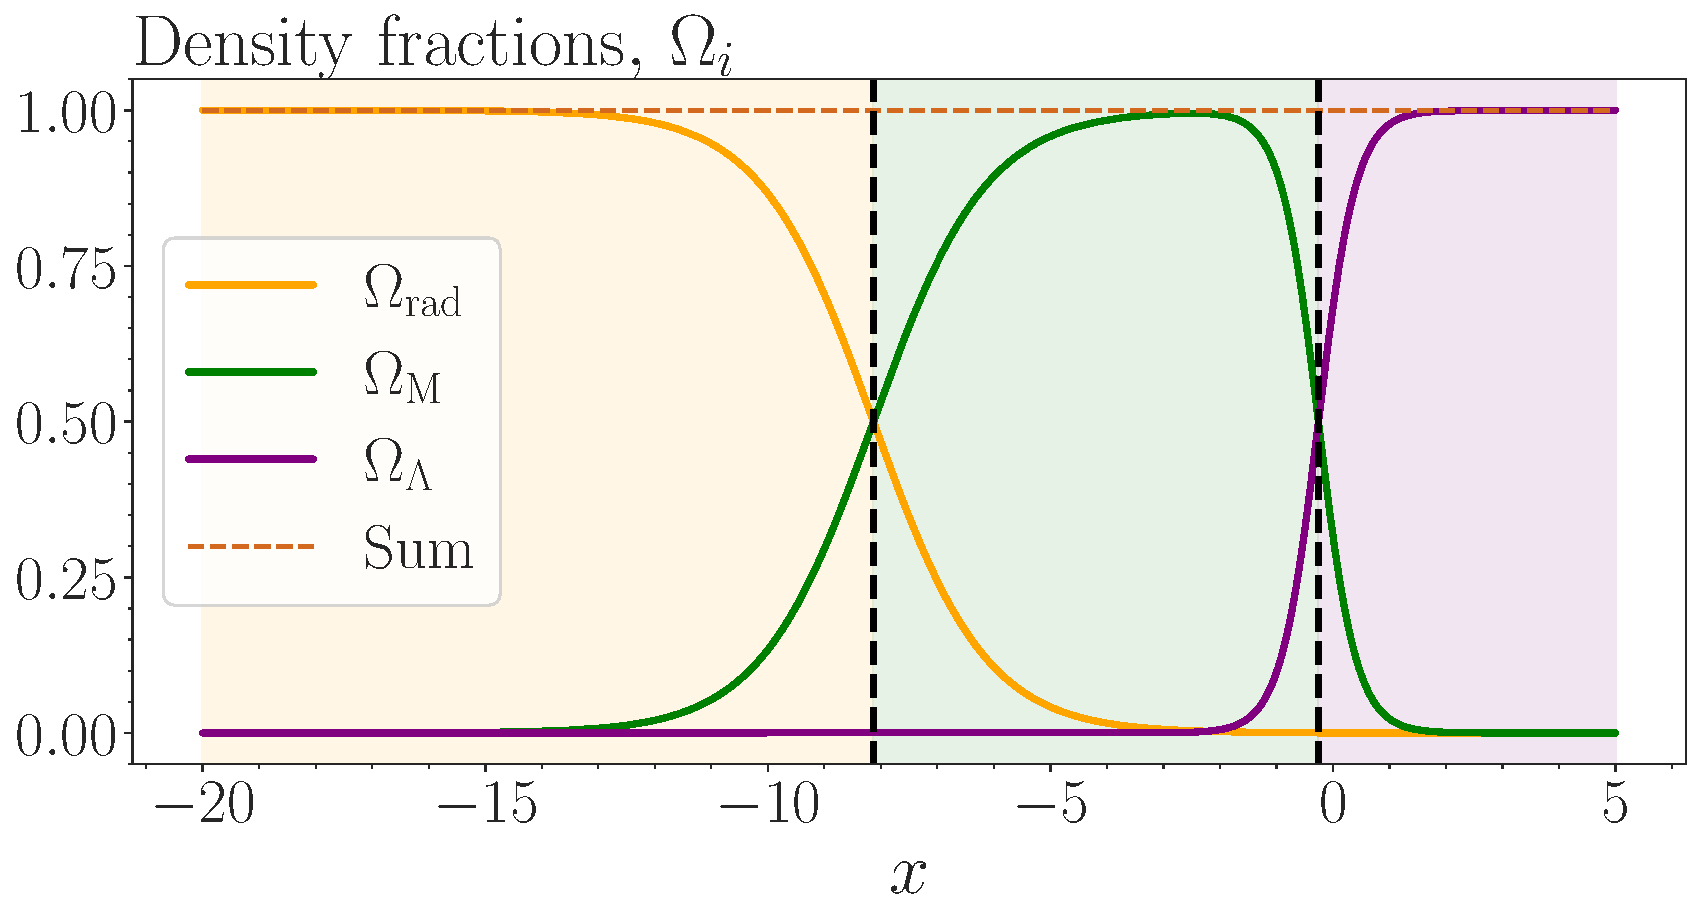
\includegraphics[width=\linewidth]{testing_omegas.pdf}
        \caption{Density fractions $\O_i$ as function of $x$. For low $x$, radiation dominates, before matter dominates and dark energy has just become the dominant energy density today $x=0$, and will continue to dominate into the future. The sum of densities sums to one across all times, as required (white dotted line). The black dotted lines are the radiation-matter equality at $x=-8.13$ and the matter-dark energy equality at $x=-0.26$, both stated in ~\cref{tab:m1:important_values}. The domination of each regime is shown as a shaded background with similar colour as its respective graph. }
        \label{fig:m1:omega_tests}
    \end{figure}
    \cref{fig:m1:eta_tests} is the sanity check for $\eta$ showing that its derive take the desired value of $c/\Hp$.
    
    
    % \TODO{fix this}
    % As explained in section ~\cref{sec:m1:theory:sanity}, we have analytical solutions for constructions of $\eta$ and $\Hp$ in the different regimes. \cref{fig:m1:eta_tests} is the sanity check for $\eta$, showing $\eta\Hp/c$ converging to finite values in the radiation and matter dominated eras (where $\alpha_{\mathrm{rad}, \mathrm{M}}>0$), and diverging towards $+\infty$ in the dark energy dominated era ($\alpha_\Lambda =-2 <0$). This is in accordance with the analytical solutions. The different regimes are shown in shaded colour. It is also worth noticing that $(\d \eta /\d x)\Hp/c$ is one for all regimes, as expected from equation ~\cref{eq:m1:theory:measures:eta_diffeq}. \TODO{to this}

    \begin{figure}
        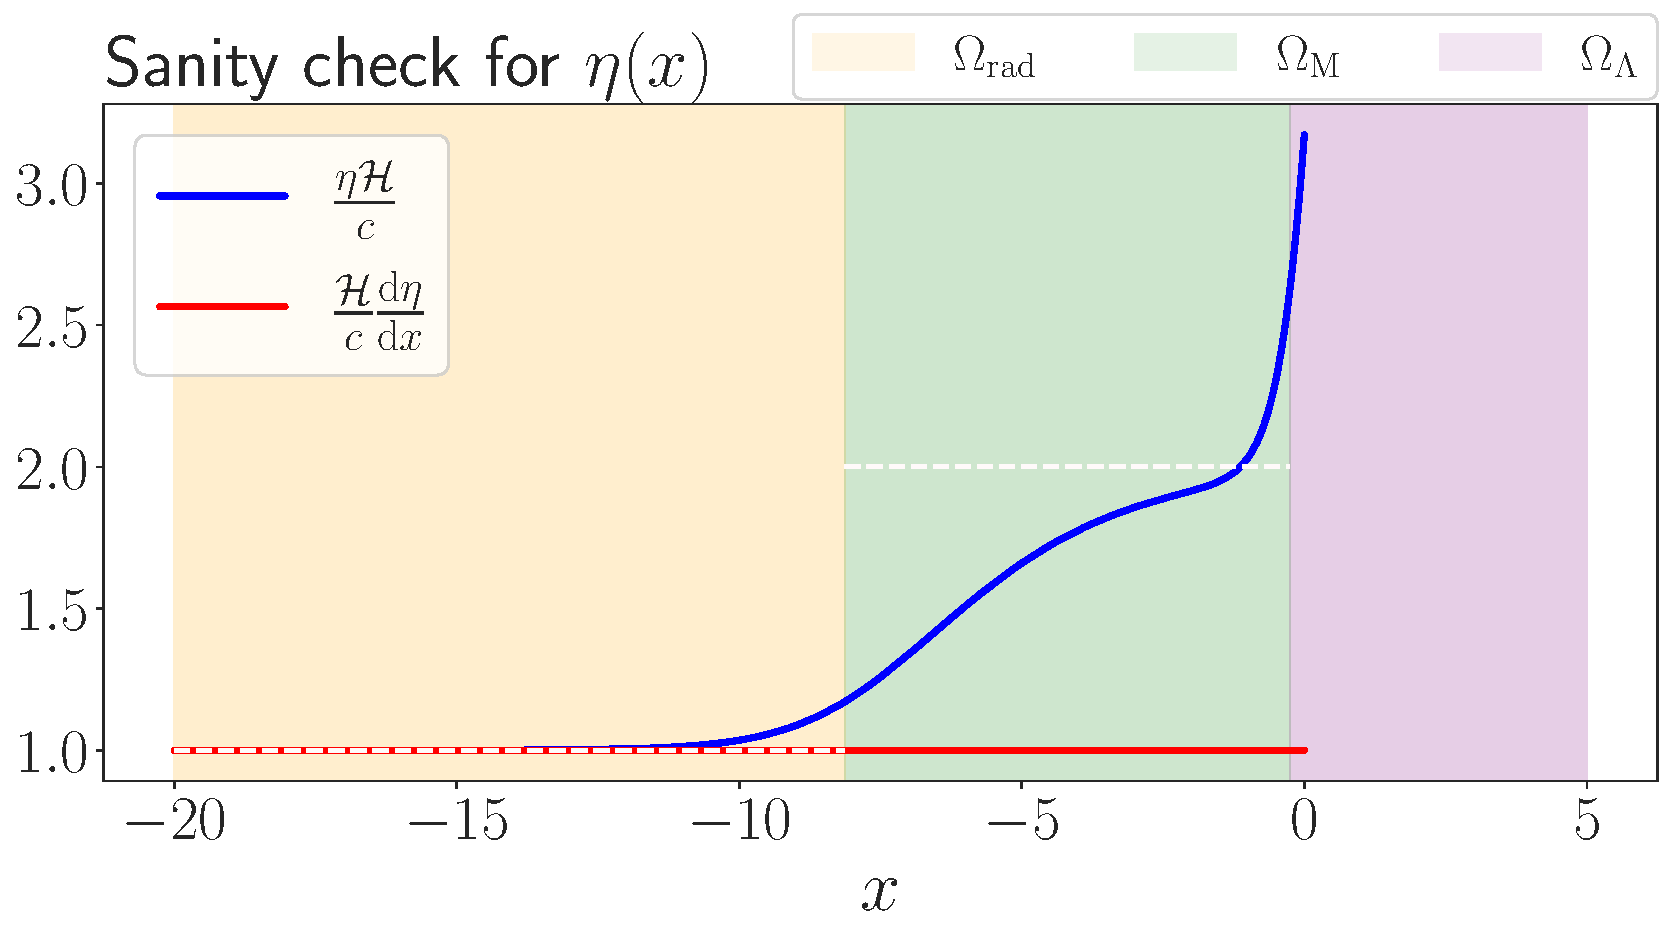
\includegraphics[width=\linewidth]{eta_test.pdf}
        \caption{Sanity check for $\eta$.}
        \label{fig:m1:eta_tests}
    \end{figure}

    ~\cref{fig:m1:Hp_tests} is the sanity check confirming that our constructions of $\Hp$ and its derivatives converge to the analytical approximation in the different regimes. The second derivative, as shown in blue, takes the value of 1 in the radiation regime, 1/4 in the matter regime and 1 in the dark energy regime. Similarly, the first derivative, as shown in red, take the value -1 in the radiation regime, -1/2 in the matter regime and 1 in the dark energy regime. This is well in accordance with the analytical approximations put forth in section ~\cref{sec:m1:theory:sanity}. 

    \begin{figure}
        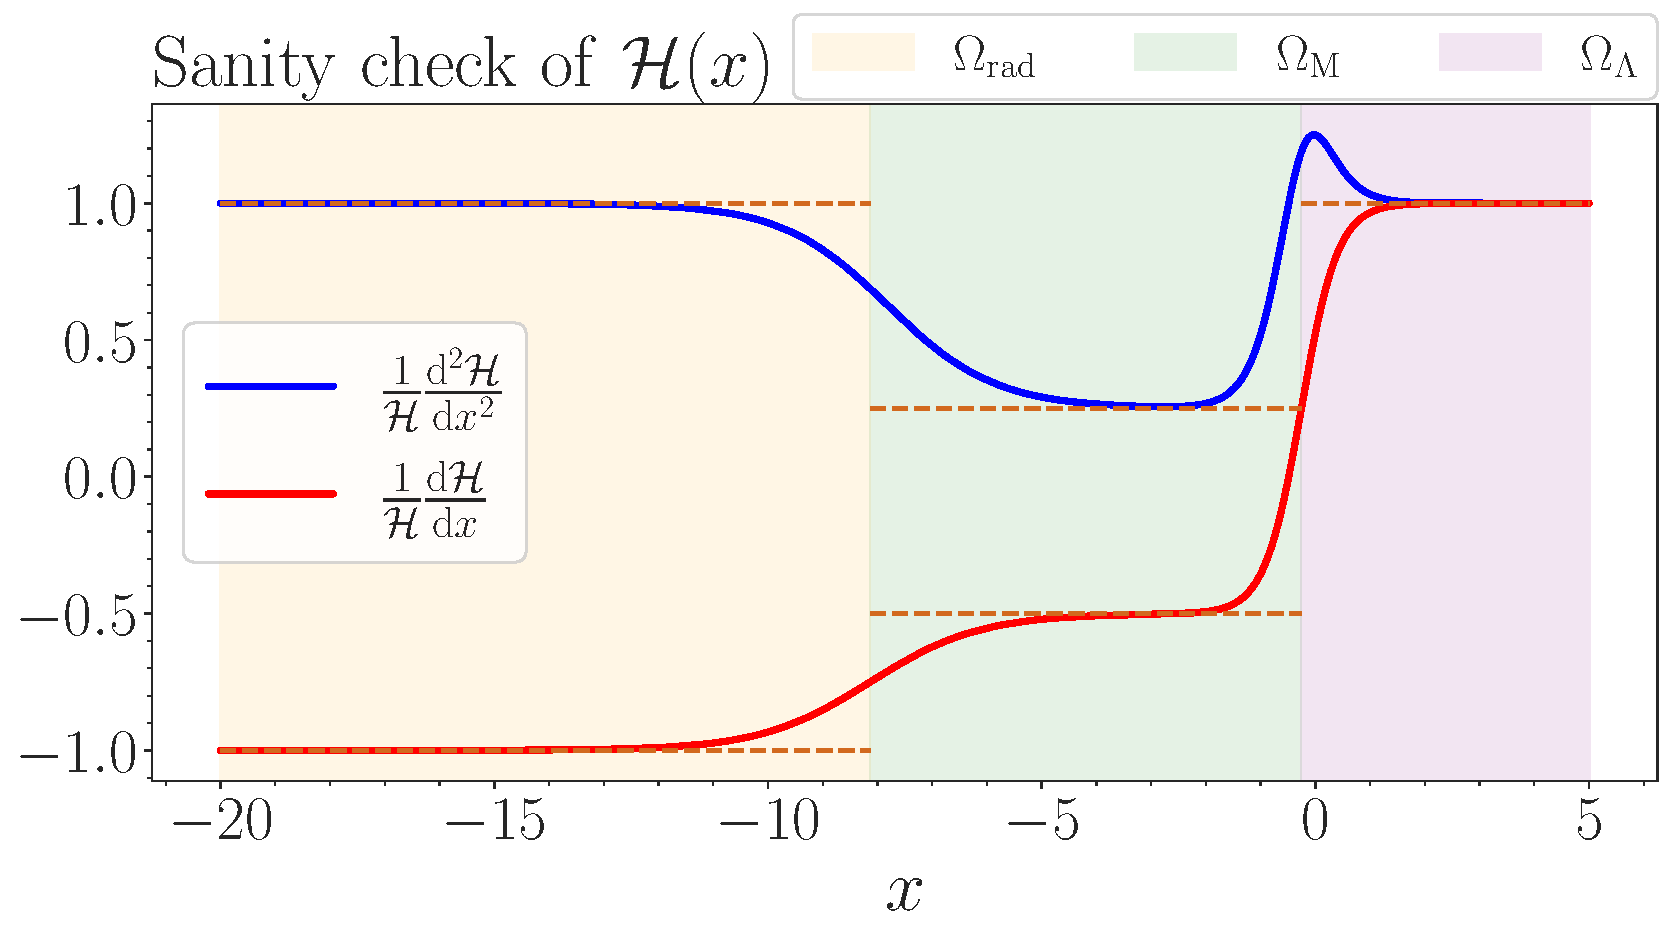
\includegraphics[width=\linewidth]{Hp_test.pdf}
        \caption{Sanity check for $\Hp$, showing that the second derivative (blue) converge to the analytical expressions shown as brown dotted lines in the different regimes. The first derivative (red) converge to its analytical values in the same regimes, which again are shown with a shaded colour.}
        \label{fig:m1:Hp_tests}
    \end{figure}

    These sanity checks are confirmations that the implementations yield the same result as the analytical approximation in the different regimes for various constructions of $\eta$ and $\Hp$ and their derivatives.
    
\subsubsection{Analysis}

    In ~\cref{sec:m1:lambdaCDM} we indicate how we can calculate the radiation-matter equality (RM-equality), matter-dark energy equality (ML-equality), when the acceleration of the universe started, the age of the universe and the conformal time today. The result is shown in ~\cref{tab:m1:important_values}. We note that the equalities is in accordance with the sanity checks, and the age of the universe today (in cosmic time) is about 13.9 Gyr. We also note that the acceleration onset is slightly before the matter-dark energy equality at $x=-0.49$ and $x=-0.26$ respectively. 
    \begin{table}
        \begin{tabular}{lrrrl}
Quantity & x & z & t [Gyr] &  \\
RM-equality  & -8.13 & 3400.33 & 0.000051 &   \\
ML-equality  & -0.26 & 0.29 & 10.378200 &   \\
Accel. start  & -0.26 & 0.29 & 10.378200 &    \\
Age of universe  & 0.00 & 0.00 & 13.857700 &   \\
Conformal time  & 0.00 & 0.00 & 46.318700 &   \\
\end{tabular}

        \caption{Important quantities in the evolution of the universe. RM stands for radiation-matter and ML for matter-dark energy.}
        \label{tab:m1:important_values}
    \end{table}

    The conformal Hubble factor, $\Hp$, is plotted against time, $x$, in ~\cref{fig:m1:conformal_hubble_factor_Hp}. It is decreasing in the radiation and matter regimes and increasing in the dark energy regime, switching signs at the acceleration onset, which is marked with a black dotted line in the figure. 
    \begin{figure}
        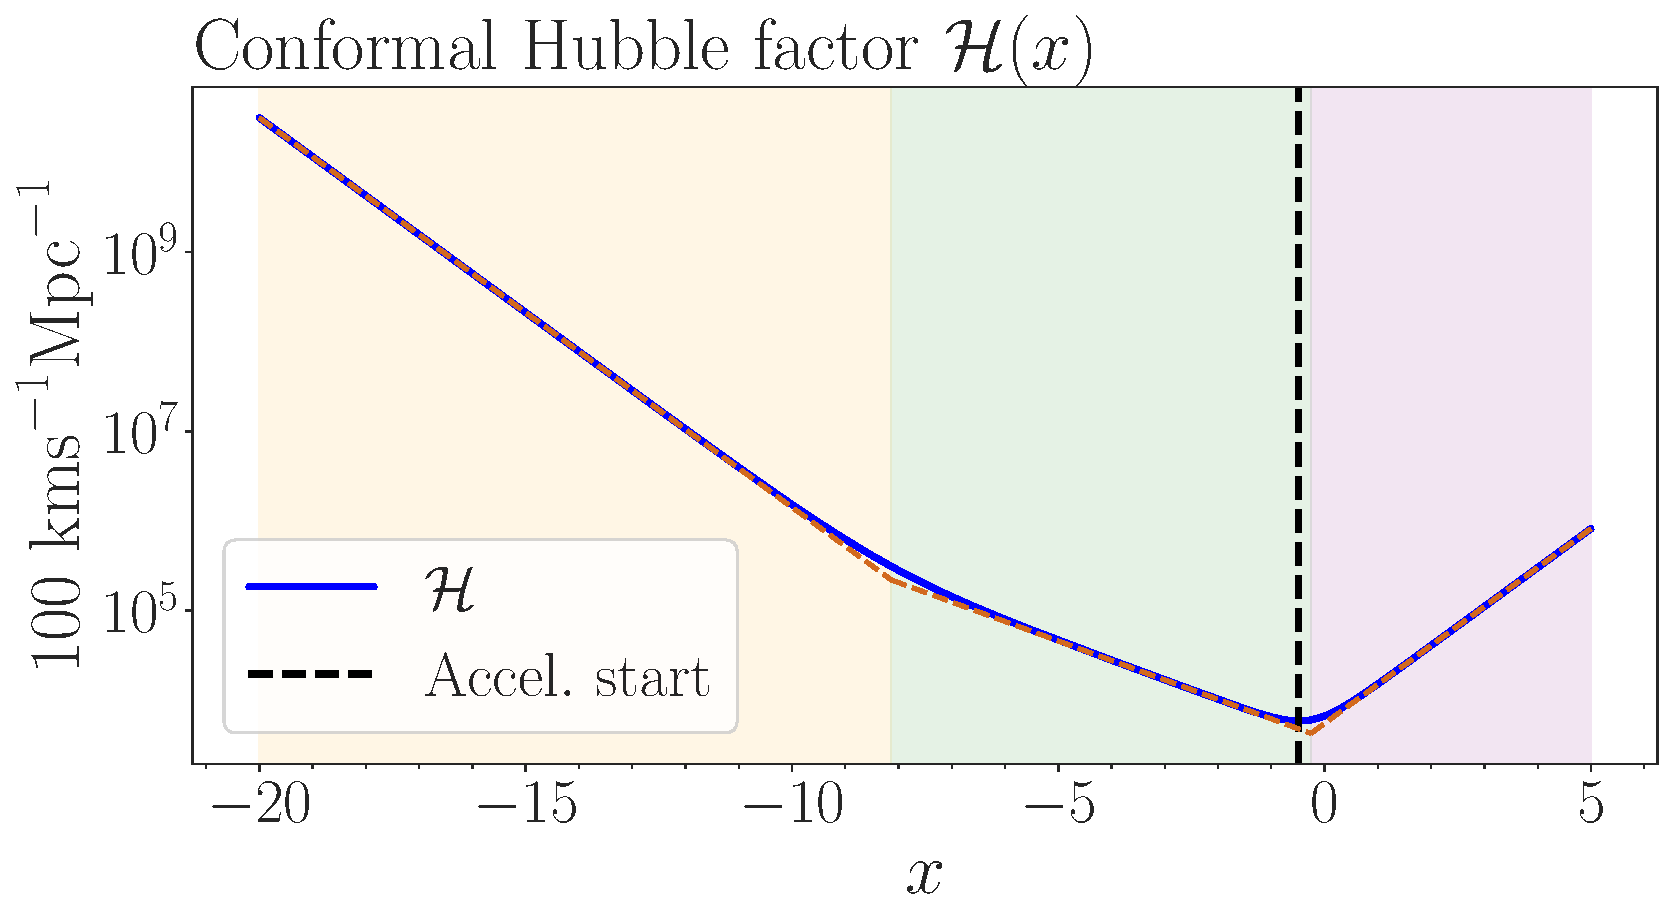
\includegraphics[width=\linewidth]{conformal_hubble_factor.pdf}
        \caption{$\Hp$ as function of $x$. It is decreasing in the radiation and matter regimes, and increasing in the dark energy regime, tightly following its analytical approximation in each regime.}
        \label{fig:m1:conformal_hubble_factor_Hp}
    \end{figure}

    ~\cref{fig:m1:cosmic_conformal_time} show the cosmic time $t$ and the conformal time $\eta/c$. The cosmic time is the age of the universe at any given time/size $x$. The low values for the cosmic time at early times suggest a rapid increase of the size of the Universe in a short cosmic time. This is supported by the conformal Hubble factor in ~\cref{fig:m1:conformal_hubble_factor_Hp} which is large for low $x$. The expansion rate of the universe decelerates until the acceleration onset, from which it accelerates. This acceleration means that the rate of expansion of the Universe will at some point surpass the conformal horizon, effectively decreasing the observable Universe. 

    \begin{figure}
        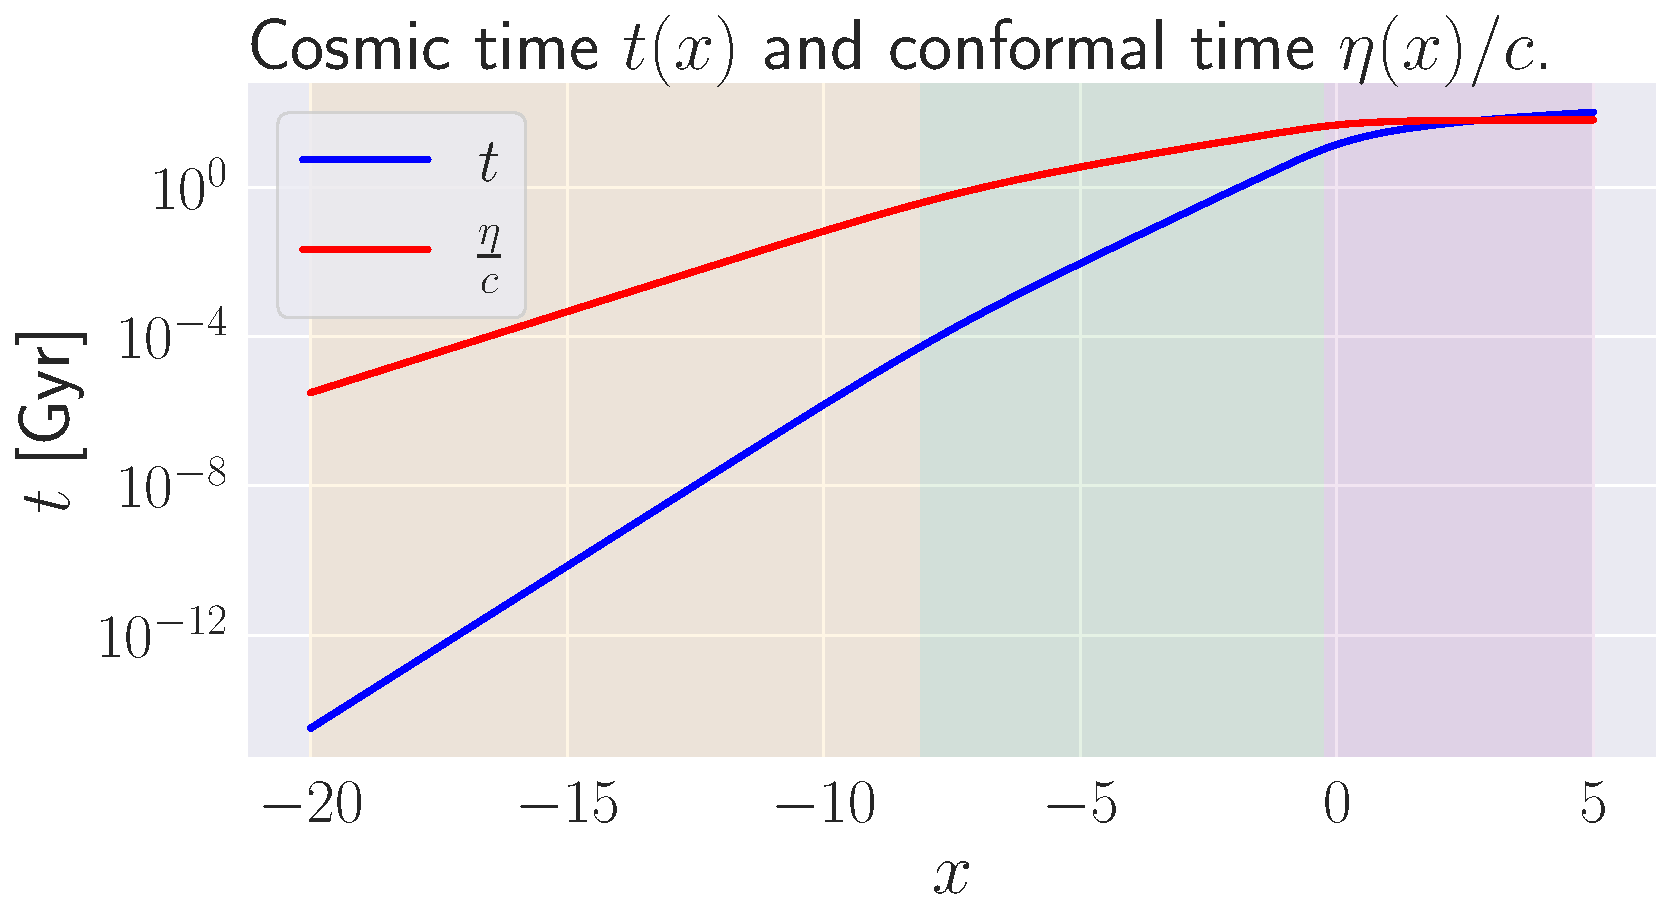
\includegraphics[width=\linewidth]{cosmic_conformal_time.pdf}
        \caption{Cosmic time (in blue) and conformal time (red).}
        \label{fig:m1:cosmic_conformal_time}
    \end{figure}

    The results of the supernova fitting, outlined in section ~\cref{sec:m1:methods:fit}, is summarised in ~\cref{tab:m1:best_fit_values}. The parameter values that maximises the likelihood (minimising) $\chi^2$ are: $h=0.702$, $\O_\mathrm{M0} = 0.259$ and $\O_{k0} = 0.274$. We also compute the posterior probability distribution function obtained from ~\cref{eq:m1:methods:fit:posterior_prob} which we have assumed to be normally distributed. From this we obtain a mean value, but also a $1\sigma$ confidence interval, which are:
    \begin{equation}\label{eq:m1:results:posterior_results}
        \begin{split}
            h &= 0.701\pm0.006 \\
            \O_\mathrm{M0} &= 0.247\pm0.110 \\
            \O_{k0} &= 0.107 \pm 0.274
        \end{split}
    \end{equation}
    
    \begin{table}
        \begin{tabular}{l|rrr}
      & $h$ & $\O_\mathrm{M0}$ & $\O_{k0}$  \\
    \hline
    Best: $\min{\chi^2}$  & 0.702 & 0.259 & 0.067  \\
    Posterior  & 0.701 & 0.247 & 0.107   \\
    $1\sigma$ confidence  & 0.006 & 0.110 & 0.274 \\ 
    \hline
    \hline
\end{tabular}
        \caption{Best and fitted values. The best fit values are those that actually minimise the $\chi^2$-value, which consequently are the most probable values. The fitted values are obtained as the mean and standard deviations of the posterior pdfs of the parameters respectively. }
        \label{tab:m1:best_fit_values}
    \end{table}
    Let's first see for ourselves if these values make sense or not, just with by-eye comparison.~\cref{fig:m1:supernova_data} shows the supernova data as red error bars, with the predictions from the fiducial cosmology plotted above it, alongside the best fit parameter values. The quantity plotted is the luminosity distance divided by redshift, $d_L/z$ for better comparison. We notice the accordance between the two, and also note that the $x$-axis in this plot is the redshift $z$ instead of the logarithm of the scale factor. This means that earlier times are to the right in the plot (high redshift), as opposed to the other plots. Immediately we see that the best fit parameters seems to do a better job at staying within the red error bars. However, the fiducial cosmology is also quite good. Furthermore, the fiducal cosmology stays well within the $1\sigma$ confidence interval found from the posterior pdfs. It is also worth noting that the uncertainties on some observed values are quite large. 

    \begin{figure}
        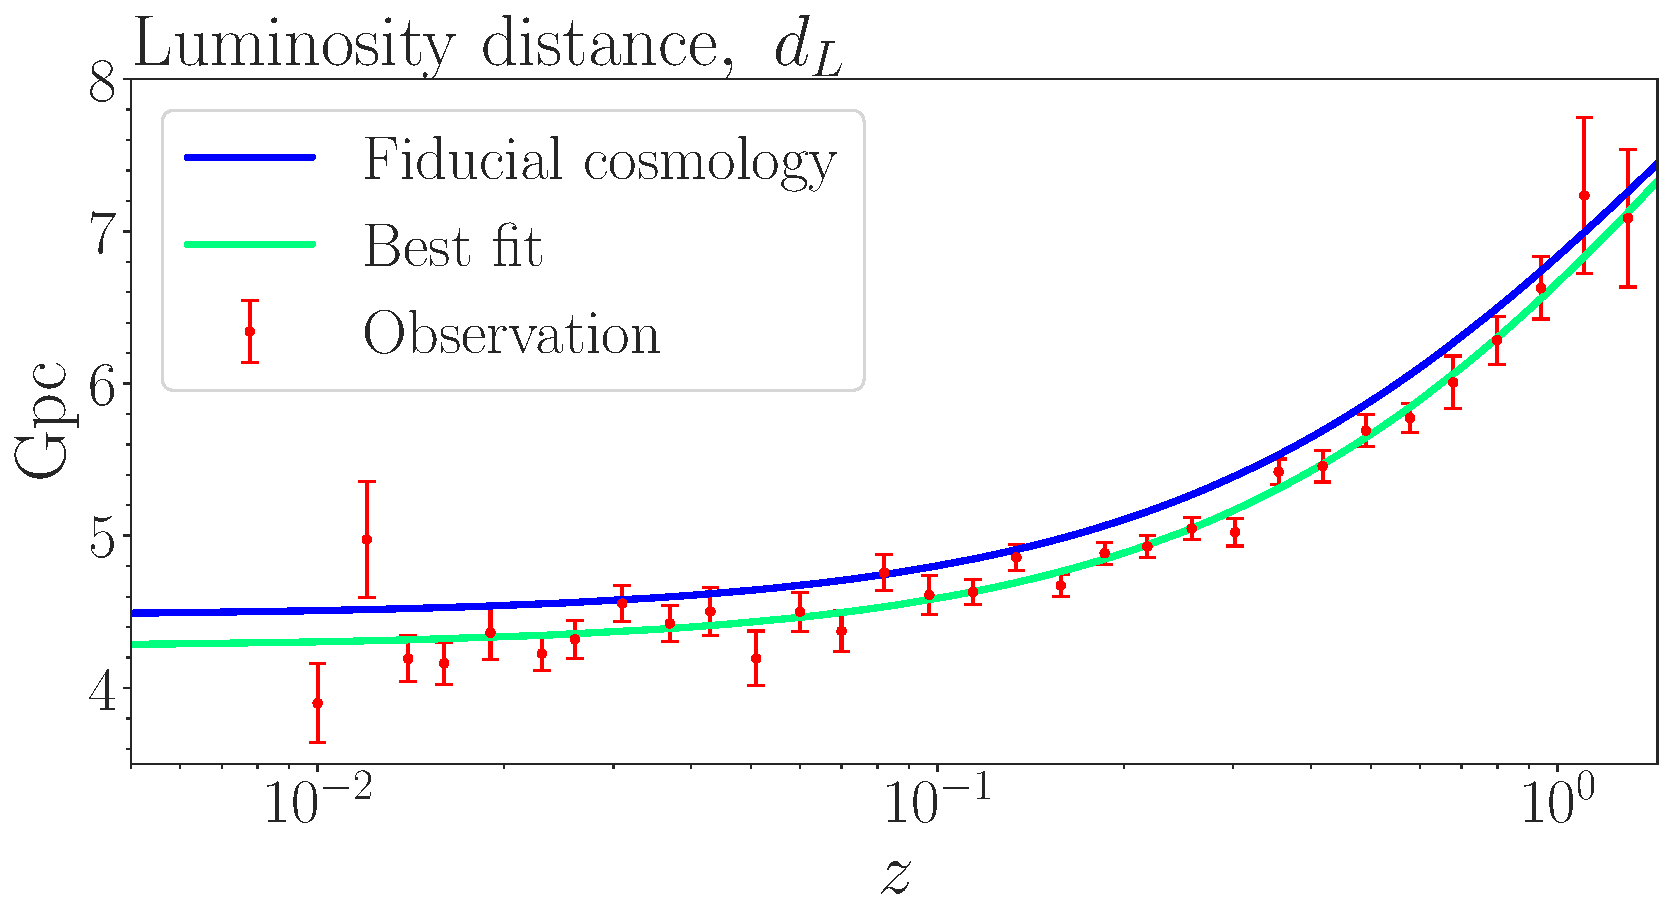
\includegraphics[width=\linewidth]{supernova_data.pdf}
        \caption{The luminosity distance predicted using the fiducial cosmology in blue, against observations of actual supernovas in red (or rather the confidence interval of the observations). The green line is found from computing the luminosity distance using a cosmology of the best fit parameters from the supernova fitting; $h=0.702, \O_\mathrm{b0} = 0.05, \O_\mathrm{CDM0} = 0.209, \O_\mathrm{k}=0.067, N_\mathrm{eff}=3.046, T_\mathrm{CMB}=2.7255 \text{K}$. Notice the $x$-axis is now the redshift $z=e^x-1$.}
        \label{fig:m1:supernova_data}
    \end{figure}

    Now let's turn to how we have constrained the parameters. ~\cref{fig:m1:omega_planes} shows the $\chi^2$-values found from ~\cref{eq:m1:methods:fit:chi2}, constrained to 1$\sigma$ interval. The black dotted line represent a flat universe, where the matter and dark energy are the main constituents of the universe. The supernova data originate in close temporal proximity to us, we thus assume that the contribution from the radiation density is negligible for making constraints on $\O_\mathrm{M0}$ and $\O_{\Lambda0}$ today. Having only $\O_\mathrm{M0}$, $\O_{\Lambda0}$ and $\O_{k0}$, where only two of them are free yield: $\O_{k0}=1-(\O_\mathrm{M0}+\O_{\Lambda0})$, which fixes the relationship, so that it does not really matter which two of them we constrain, as the constraint on the third automatically follows.\footnote{This is why we are able to put constraints on $\O_{\Lambda0}$ even though this parameter is not (directly) sampled in the MCMC sampling.}
    
    \begin{figure}
        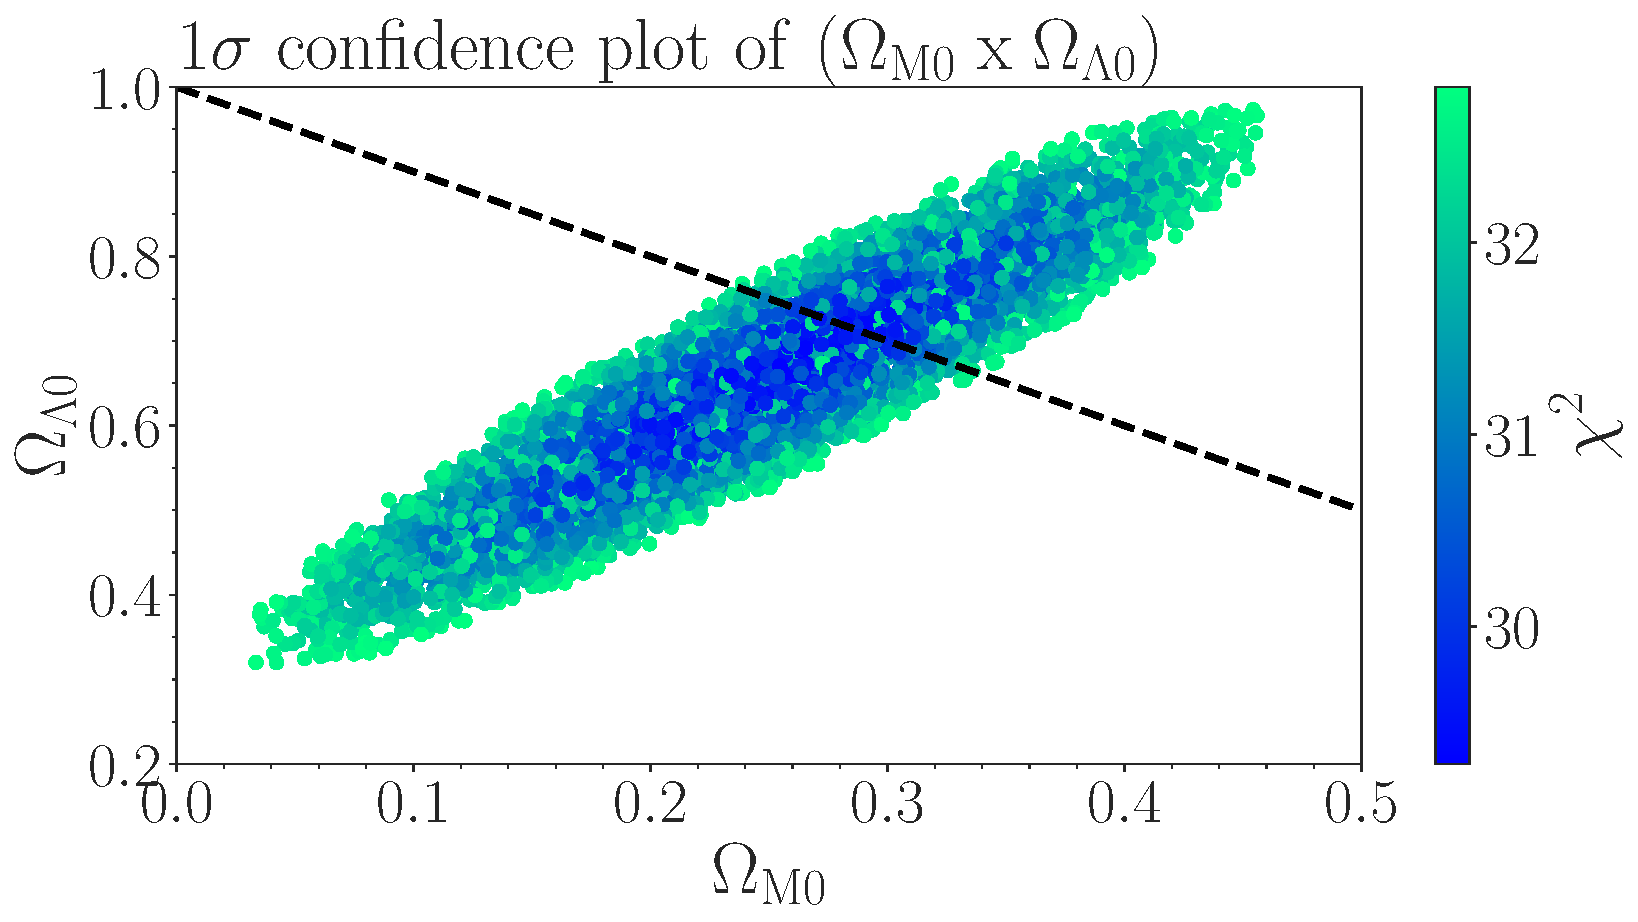
\includegraphics[width=\linewidth]{omega_plane.pdf}
        \caption{Scatter plot showing the $\chi^2$-values of the luminosity distance $d_L$ between the observed values $\mathcal{D}$ and the sampled values, as function of $\O_\mathrm{M0}$ and $\O_{\Lambda0}$. The data shown is the $1\sigma$ confidence region. The black dotted line signifies a flat universe. }
        \label{fig:m1:omega_planes}
    \end{figure}
    
    From the sampled values we then generate the posterior pdf by making a histogram of all the samples. This is seen for $\O_\mathrm{M0}$ and $\O_{k0}$ in ~\cref{fig:m1:posterior_pdf_omega_m_k} and for $H_0$ in ~\cref{fig:m1:posterior_pdf_H0}, all histograms are in turquoise. From the samples we also find their respective mean and standard deviation, from which we plot a green Gaussian curve on top of the histogram. The means are indicated with black dotted lines, and the $1\sigma$ confidence regions are shaded in blue. Both quantities are also stated in text in each plot, inn accordance with those presented in ~\cref{tab:m1:best_fit_values}. From inspection, we see that the histograms are quite close to being normally distributed, so the fitted Gaussian is quite a good fit. 
    
    \begin{figure}
        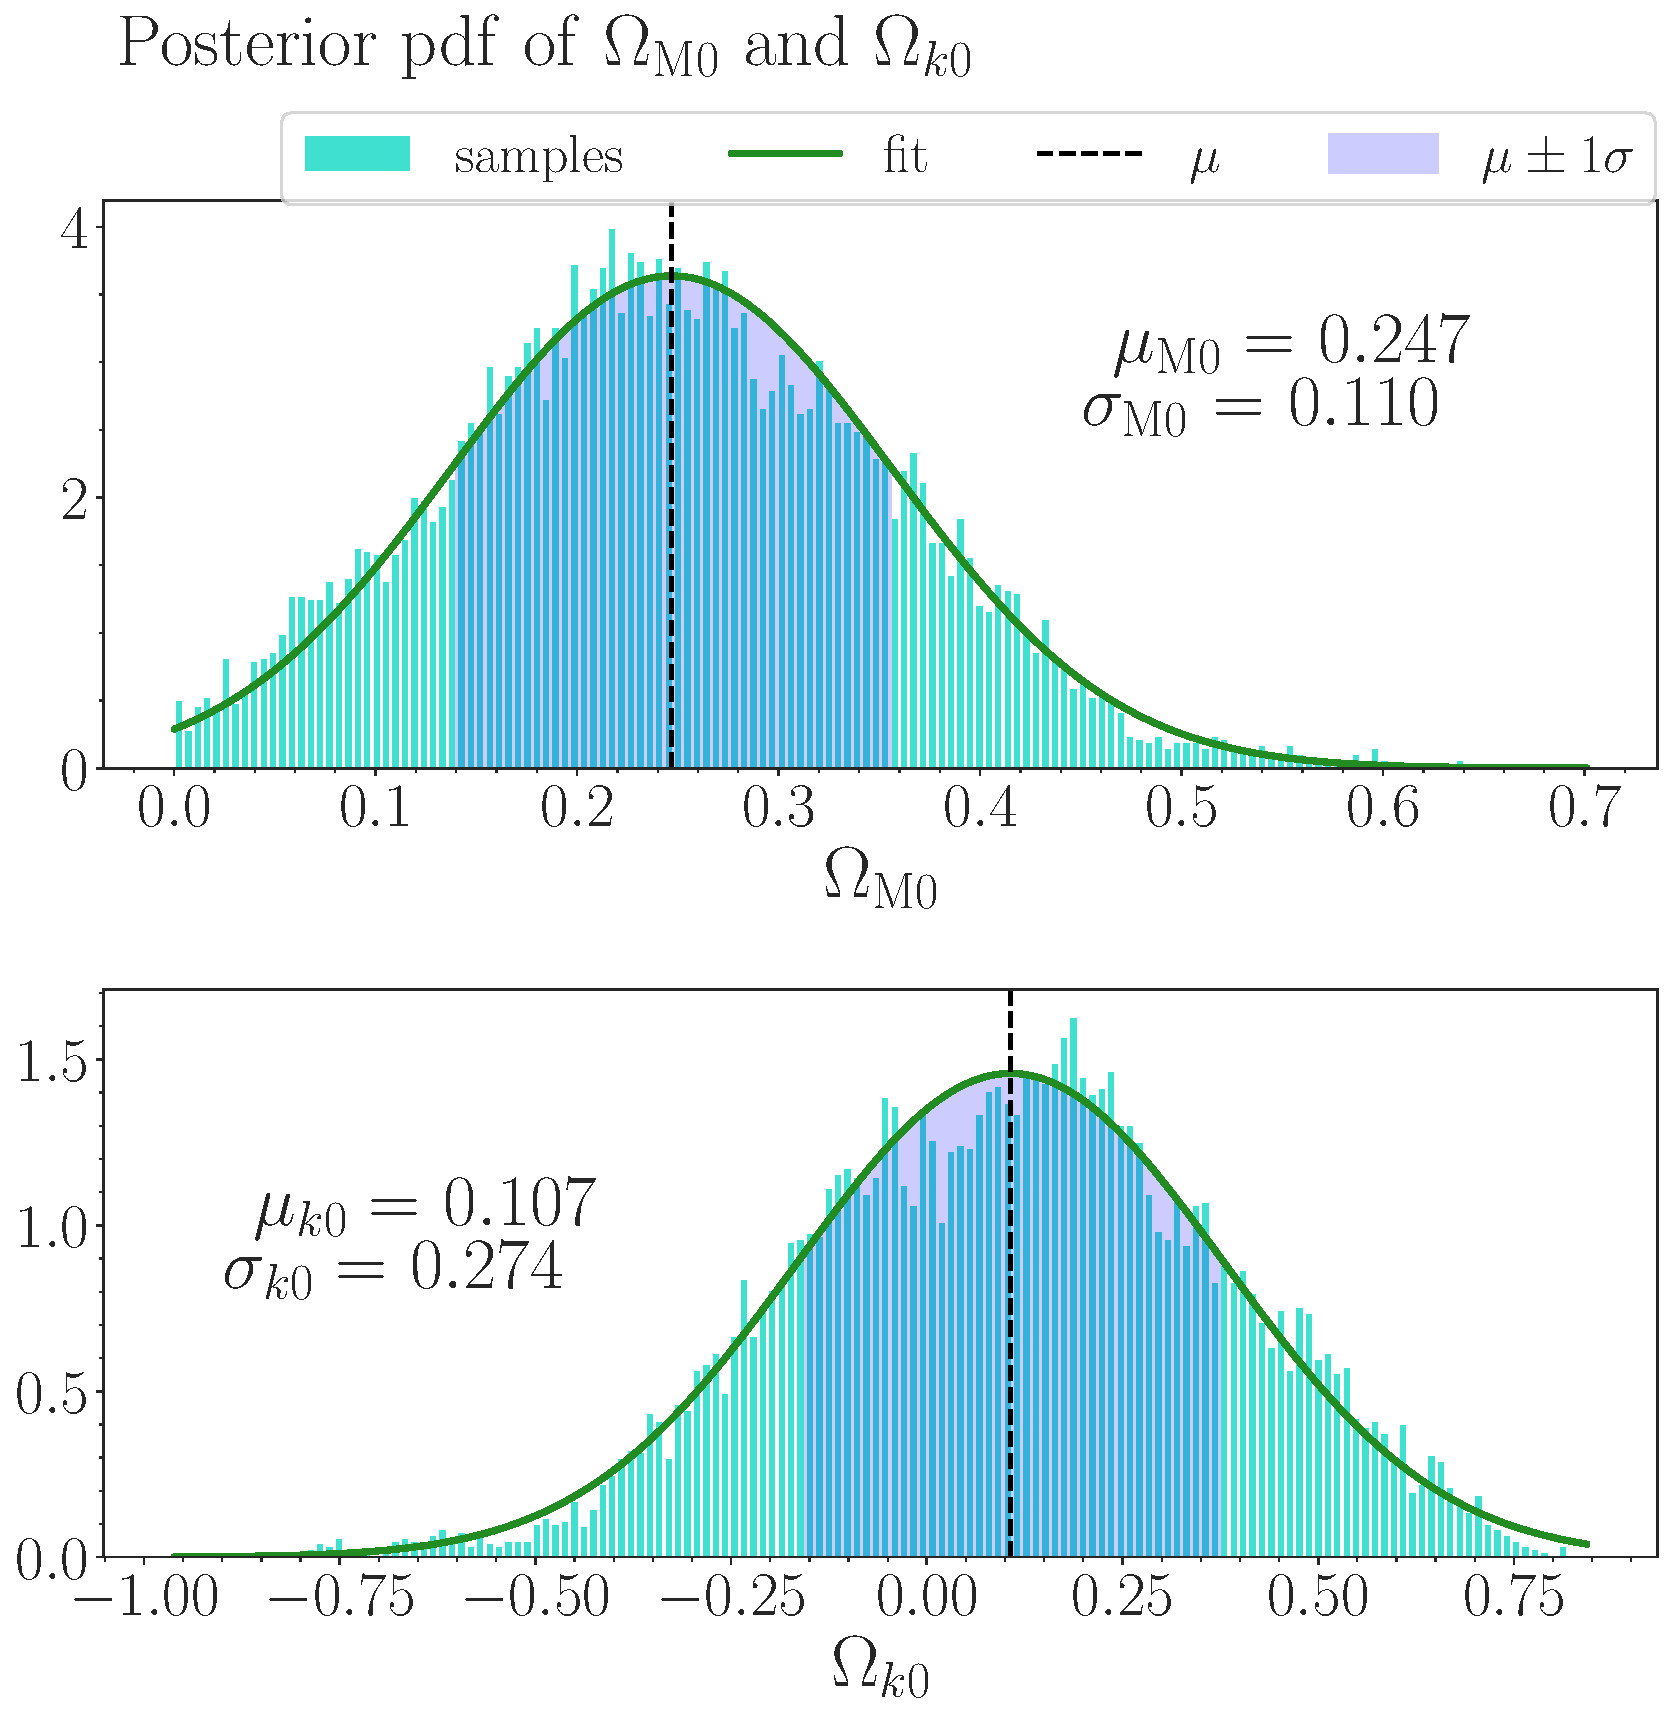
\includegraphics[width=\linewidth]{probs_M_K.pdf}
        \caption{Posterior probability distributions (pdfs) of $\O_\mathrm{M0}$ and $\O_\mathrm{k0}$ as result of the MCMC sampling. The samples are shown in turquoise and the constructed pdfs in green. The mean $\mu$ is shown as a black dotted line, with the $1\sigma$ confidence interval in shaded blue ($\mu\pm 1\sigma$)}
        \label{fig:m1:posterior_pdf_omega_m_k}
    \end{figure}
    
    \begin{figure}
        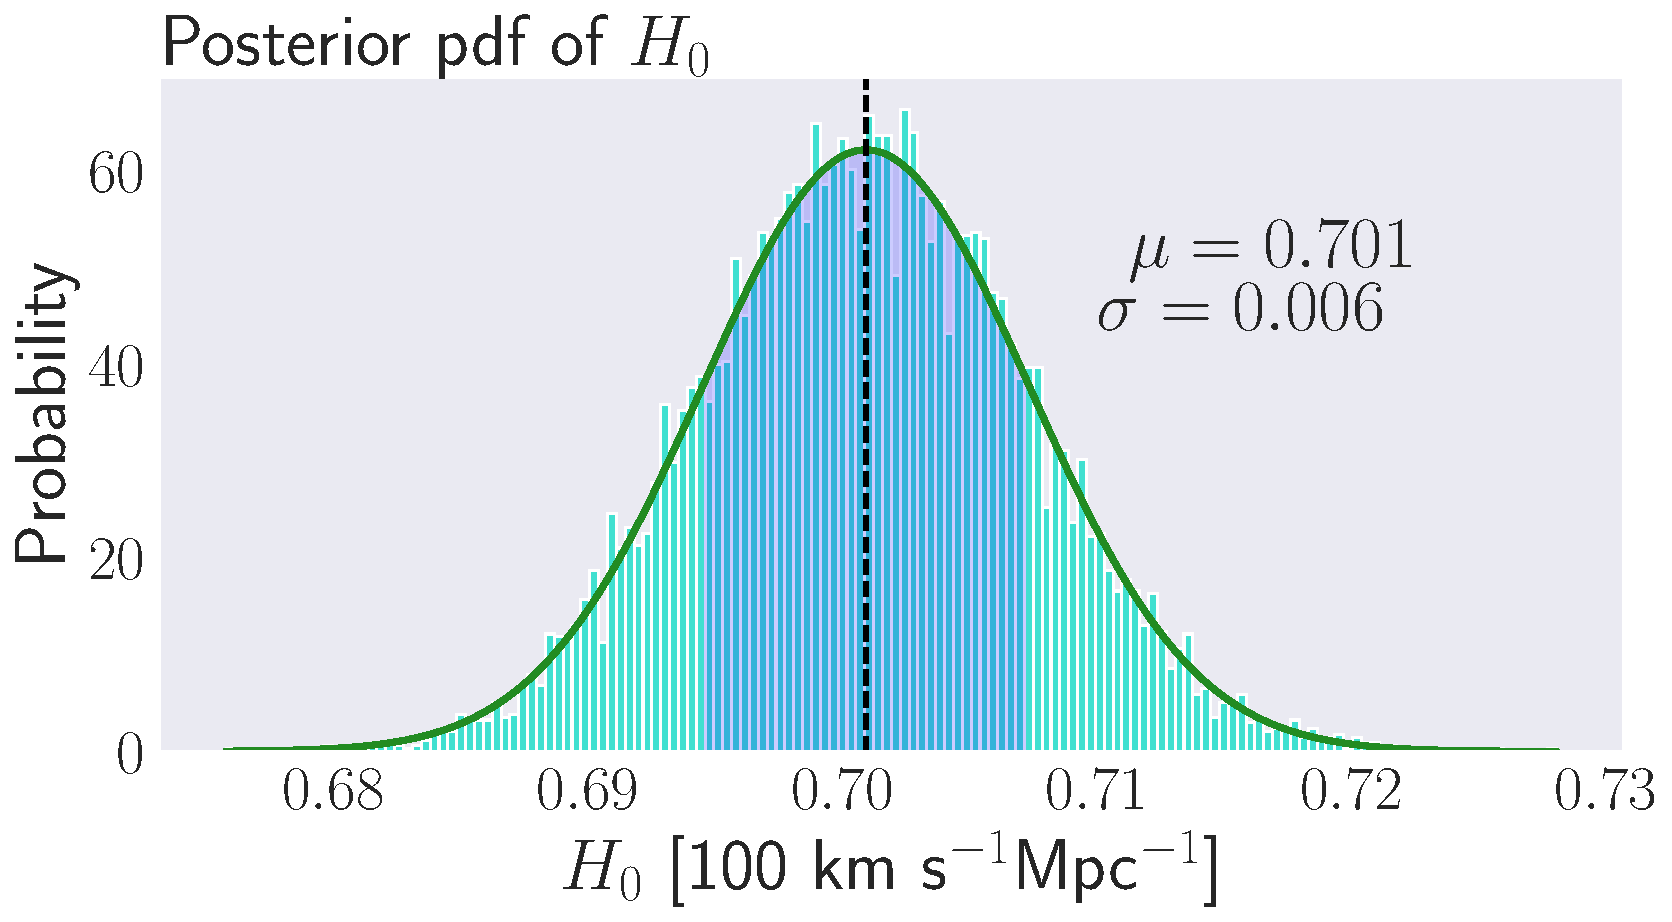
\includegraphics[width=\linewidth]{posterior_pdf.pdf}
        \caption{Posterior probability distribution (pdf) of $H_0$ as result of the MCMC sampling.}
        \label{fig:m1:posterior_pdf_H0}
    \end{figure}

    Discussing the goodness of the fit further, we may turn to the criterion from ~\cref{eq:m1:fit:goodness_of_fit}. ~\cref{fig:m1:goodness_of_fit} show a histogram of the sampled $\chi^2$ values, divided by $N$. In sight of prior discussion, the mean value of $\chi^2/N$ is 1.052, which is not that much larger than 1. Thus, we deduce that the fit is quite good. Although we also see from the figure that $\chi^2/N$ deviates significantly from the Gaussian curve in green.  
    
    \begin{figure}
        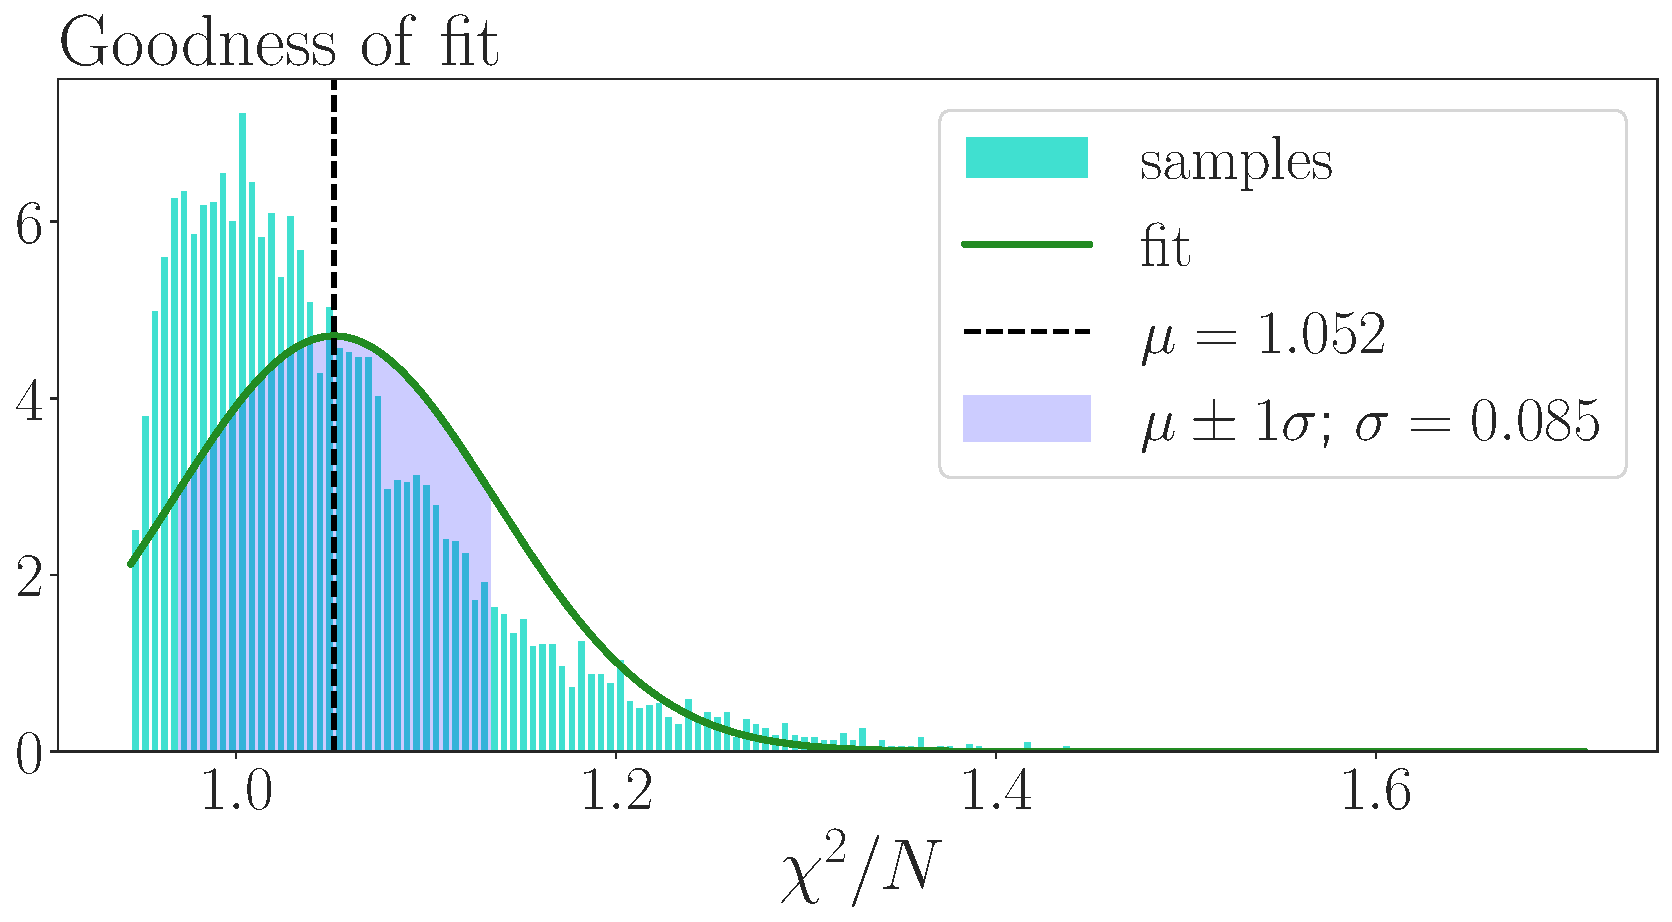
\includegraphics[width=\linewidth]{goodnes_of_fit.pdf}
        \caption{Goodness of fit, showing the mean value of $\chi^2/N$ is close to 1, which is a good fit. The Gaussian function does not seem to encapsulate behaviour of the samples. \TODO{is it really a $\chi^2$-distribution with 3 dof?. hmmm.}}
        \label{fig:m1:goodness_of_fit}
    \end{figure}

    Nevertheless, we shall continue to use the fiducial cosmology from ~\cite{Betoule_2014}, but now we have some viable constraints on them. 
    